\section{Similarity}

\subsection{Structural-Based Similarities}

Especially when analyzing long time series, similarity is computed on a structural level. We extract global features from each time series, build a feature vector from them, and measure similarity by comparing those features. Typical features are the mean and variance, the maximum and minimum, the skewness, and the mean and variance of the $1^{st}$ derivative.

A measure used to compute structural dissimilarity is \textbf{compression based dissimilarity}, defined as:
\begin{equation*}
    d(x,y) = \textit{CDM}(x,y) = \dfrac{C(x,y)}{C(x) + C(y)} \,,
\end{equation*}
where $C$ is a compression algorithm. The numerator is the compression of the two series concatenated, while the denominator is the sum of the compressions of each series taken alone. The Compression Dissimilarity Measure equals 1 when the two series are unrelated, and is less than one otherwise. The smaller its value, the closer the series are to each other, so compressing them together saves space. CDM is never zero.

\subsection{Shape-Based Similarities}

Shape-based similarities can be computed using distance measures. Recall that distances satisfy the following properties:
\begin{align*}
    &d(a,b) \geq 0,\; d(a,b) = 0 \iff a = b \ (\text{Positivity}) \\
    &d(a,b) = d(b,a) \ (\text{Symmetry}) \\
    &d(a,c) \leq d(a,b) + d(b,c) (\text{Triangle Inequality})
\end{align*}
One way to compute shape-based dissimilarity is the Euclidean distance. Given two time series with exactly the same number of points, the Euclidean distance treats each series as a point in a Euclidean space. Two series that differ sharply in shape can still look similar in terms of structural features such as maximum and minimum. This distance is very sensitive to distortions in the data, which should be removed in a preprocessing phase.\\
The most common distortions are:
\begin{itemize}
    \item \textbf{Offset translation}: the series have different offsets on the y axis. Computing the distance without addressing this problem returns a value drastically larger than the actual shape distance. We correct it by subtracting from each series its own mean value.
    \begin{figure}[h]
        \centering
        \begin{minipage}{0.40\textwidth}
        \centering
         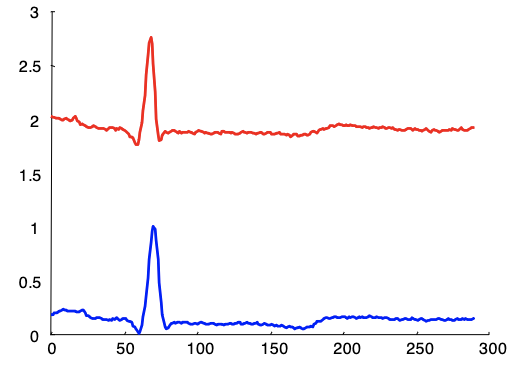
\includegraphics[width=0.8\linewidth]{img/offset_trans_1.png}
        \end{minipage}
        \hfill
        \begin{minipage}{0.40\textwidth}
        \centering
            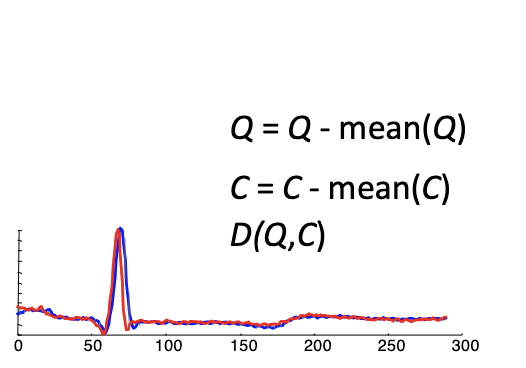
\includegraphics[width=0.8\linewidth]{img/offset_trans_2.png}
        \end{minipage}
        \label{fig:offset-trans}
        \caption{Offset translation transformation.}
    \end{figure}

    \item \textbf{Amplitude scaling}: the series have the same shape but are scaled differently on the y axis. We correct it by applying Z-score normalization to the values of each series (subtracting the mean and dividing by the standard deviation).
    \begin{figure}[h]
        \centering
        \begin{minipage}{0.40\textwidth}
               \centering
            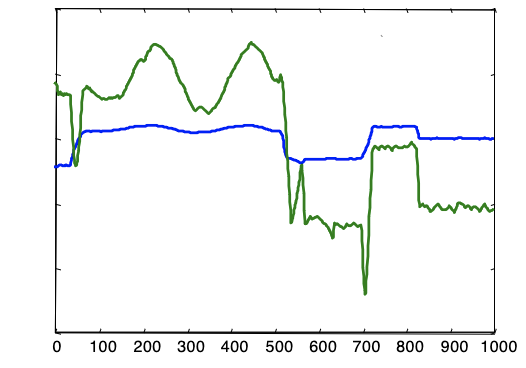
\includegraphics[width=0.8\linewidth]{img/Ampli_scaling_1.png}
        \end{minipage}
        \hfill
        \begin{minipage}{0.40\textwidth}
               \centering
            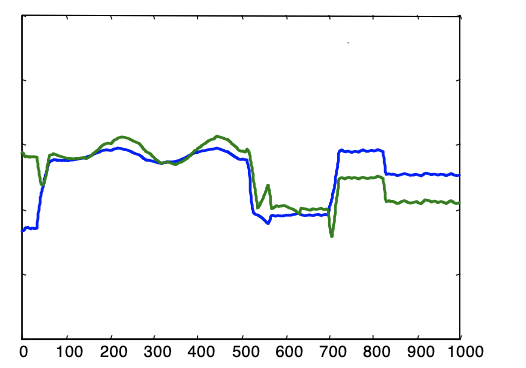
\includegraphics[width=0.8\linewidth]{img/Ampli_scaling_2.png}
        \end{minipage}
        \caption{Amplitude scaling transformation.}
        \label{fig:ampli-scaling}
    \end{figure}

    \item \textbf{Linear trend}: a series can follow an upward or downward linear trend, meaning that as it progresses it steadily increases or decreases in level. We correct it by finding the best-fitting line to the time series and subtracting that line from the series itself.
    \begin{figure}[H]
        \centering
        \begin{minipage}{0.40\textwidth}
               \centering
            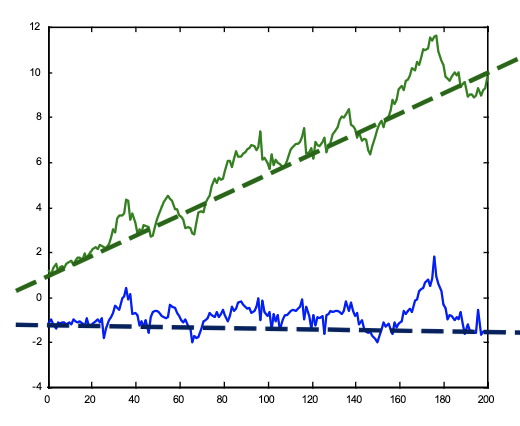
\includegraphics[width=0.8\linewidth]{img/lin_trend_1.png}
        \end{minipage}
        \hfill
        \begin{minipage}{0.40\textwidth}
               \centering
            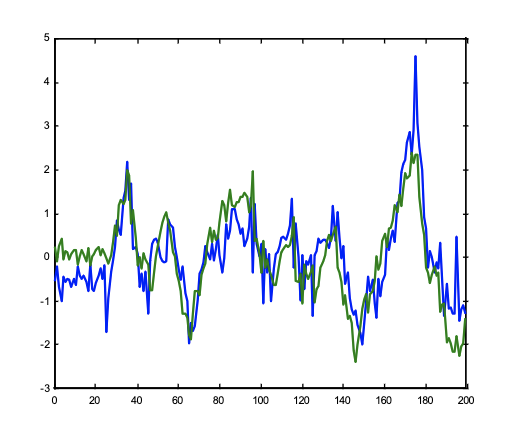
\includegraphics[width=0.8\linewidth]{img/lin_trend_2.png}
        \end{minipage}
        \caption{Linear trend transformation.}
        \label{fig:lin-trend}
    \end{figure}

    \item \textbf{Noise}: noise is random error present in the series. To reduce it, each data point can be replaced with the average value of its neighbors.
    \begin{figure}[h]
        \centering
        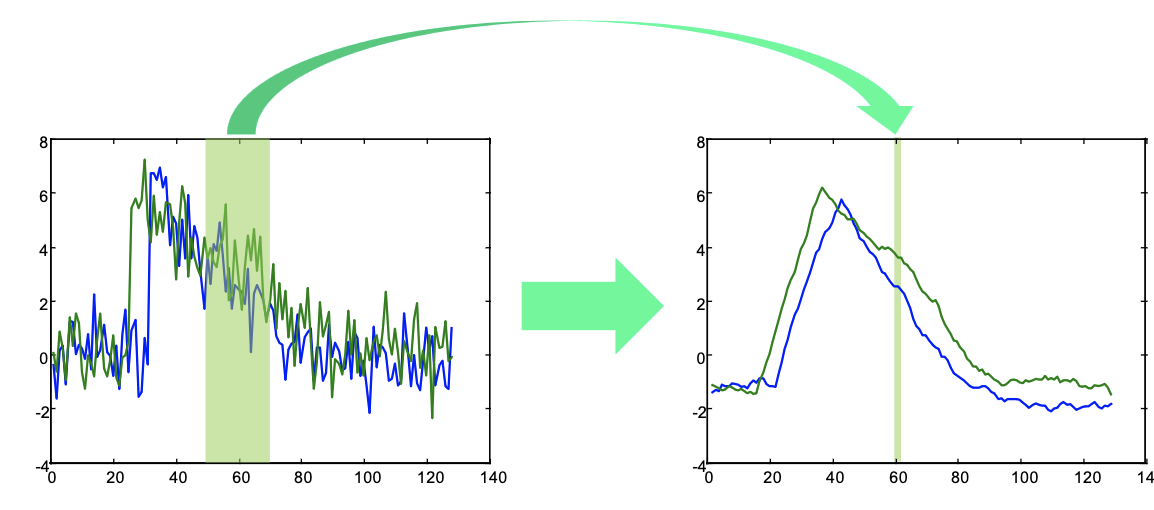
\includegraphics[width=0.8\linewidth]{img/noise_transf.png}
        \caption{Noise transformation.}
        \label{fig:noise-trans}
    \end{figure} \\
    Noise can be reduced by a \textbf{moving average} (\textbf{MA}): given a window of length $w$ and a time series $t$, the MA is applied as:
    \begin{equation*}
        t_i = \dfrac{1}{w} \sum_{j=i-(w-1)/2}^{i+(w-1)/2} t_j \ i = 1, \dots , n
    \end{equation*}
    When the window is as large as the whole series, we are extracting a single feature rather than smoothing. The moving average also drops the first observations and shortens the series, so we must inspect our data first: this technique does not fit every case.
\end{itemize}

\paragraph{Dynamic Time Warping}

Two time series often have approximately the same shape yet do not line up on the x axis. The Euclidean distance computed between such series is high despite their similarity, because it assumes a fixed time axis shared by both. To recover their similarity, the time axis must be ``warped'' for one or both series so they align correctly.

In practice, DTW is computed in three steps. First, given the series $Q$ and $C$, we build a matrix of size $|Q| \times |C|$ whose cell $i,j$ holds the distance between the $i^{th}$ component of $Q$ and the $j^{th}$ component of $C$, through $D(i,j)=|Q_i-C_j|$. The diagonal of this matrix corresponds to the comparison done by the Euclidean distance. Every possible warping between the two series corresponds to a path from the bottom left corner $(0,0)$ to the top right corner $(|Q|,|C|)$ of the matrix. The DTW is the best path, that is, the one with the lowest sum of costs. We find it recursively, using the following formula for the cost of the best path reaching $(i,j)$:
\begin{equation*}
    \gamma(i,j) = d(q_i,c_j) + \min\{\gamma(i-1, j-1), \gamma(i-1, j), \gamma(i, j-1)\}
\end{equation*}
The idea is that the best path must pass through $(i-1,j), (i-1,j-1)$ or $(i,j-1)$.
The dynamic programming approach first computes the distance matrix for the two series, then the matrix of cumulative costs, and finally traces the best alignment by connecting the cells of lowest cost.
\begin{figure}[h]
    \centering
    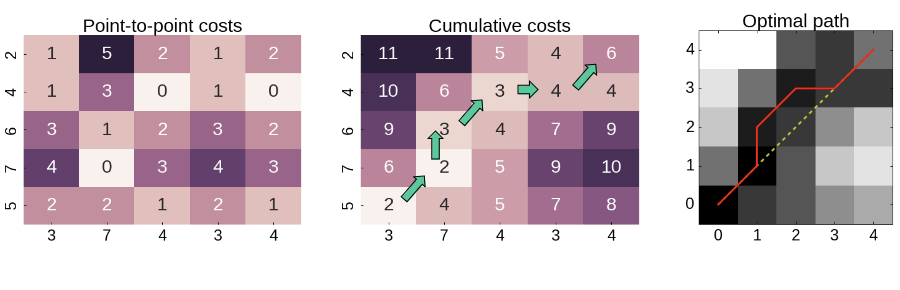
\includegraphics[width=0.9\linewidth]{img/dtw.png}
    \caption{How Dynamic Time Warping is calculated.}
    \label{fig:dtw}
\end{figure}

Comparing Euclidean distance and DTW on classification tasks, the former reaches much lower accuracy than the latter. DTW is also two to three orders of magnitude slower than Euclidean distance, which makes it unsuitable for larger datasets when used as is. To speed up its computation, we choose an approach based on the length of the time series.

\begin{itemize}
    \item If the series are short, we run DTW after searching over the warping window size, or we \textbf{approximate} the series via compression or downsampling; alternatively, we introduce \textbf{global constraints}.

    \item If the series are long and we know nothing about our data, we use compression or approximation-based dissimilarity. When we do know something about them, we extract features instead.
\end{itemize}

\paragraph{Global Constraints}

A global constraint limits the indices of the warping path $w_k = (i,j)_k$, so that $j-r \leq i \leq j+r$, where $r$ is an integer that sets the allowed range of warping for a given point in the series. This confines the computation of distances and cumulative costs to a small window of width described by $r$. Two common global constraints are the \textbf{Sakoe-Chiba Band} (restriction around the diagonal) and the \textbf{Itakura Parallelogram} (greater restriction at the extremes of the series, less in the middle). Empirical analysis shows that, on a given dataset, increasing $r$ rapidly improves performance up to a maximum, after which performance decreases and then plateaus.

\begin{figure}[h]
    \centering
    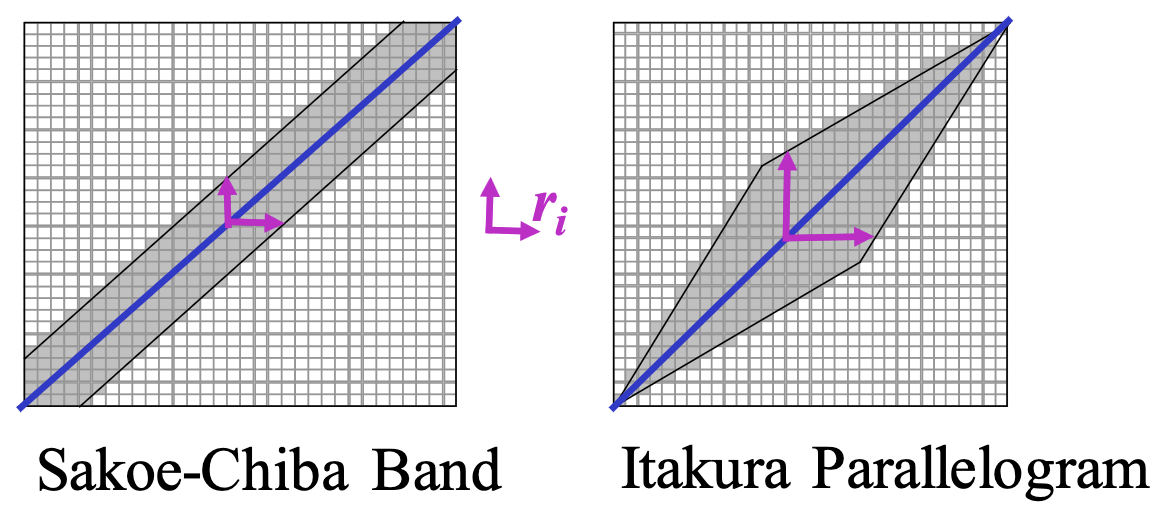
\includegraphics[width=0.5\linewidth]{img/dtw_global_constr.png}
    \caption{Global constraints.}
    \label{fig:dtw-global-constr}
\end{figure}

\paragraph{Approximation}

Approximation is a form of dimensionality reduction designed for time series; since the computations are repeated many times, approximating the data pays off. Compared to compression, approximation maps the series to a smaller space that stays interpretable, whereas the compressed space is not necessarily interpretable.

\begin{itemize}
    \item \textbf{Discrete Fourier Transform (DFT)}: the time series is represented as a linear combination of sine and cosine functions, but only the first $n/2$ coefficients are kept. Each sine wave needs only 2 numbers: the phase ($w$) and the amplitude ($A,B$). A series represented with DFT is said to be in the frequency domain. Many coefficients have very low amplitude and contribute little to the reconstructed signal, so they can be discarded with no significant loss of information, saving storage space.

    This approximation works well for most time series that represent natural signals, and many fast ($O(n \log(n))$) implementations exist. It struggles with series of different lengths and cannot support weighted distance measures. It also loses the temporal information of the original series, so we are limited to Euclidean distance.

    \item \textbf{Discrete Wavelet Transform (DWT)}: the time series is represented as a linear combination of wavelet basis functions, but only the first $N$ coefficients are kept ($N < n$). Wavelets represent data as sums and differences of a prototype wavelet, called the analyzing or mother wavelet; they are localized in time, so some wavelet coefficients represent small subsections of the data rather than the whole series, unlike Fourier coefficients, which always capture a global contribution.

    This approximation compresses stationary signals well, and many fast ($O(n)$, linear time) implementations exist. It can be defined only for sequences whose length is an integral power of two, it tends to approximate the left side of the sequence at the expense of the right, and it cannot support weighted distance measures. It also loses the temporal information of the original series.

    \item \textbf{Singular Value Decomposition (SVD)}: the time series is represented as a linear combination of eigenwaves, but only the first $n$ coefficients are kept. This approach resembles the previous two, except that the eigenwaves are extracted from the data rather than fixed in advance, so they are data dependent.

    We can think of time series as points in a high-dimensional space and rotate the axes so that axis 1 aligns with the direction of maximum variance, axis 2 aligns with the direction of maximum variance orthogonal to axis 1, and so on until the desired number of axes is reached. Since the first eigenwaves capture the most variance in the data, the rest can be truncated with little loss. This approximation loses the temporal information of the original series.

    \item \textbf{Piecewise Linear Approximation (PLA)}: the time series is represented as a sequence of $k$ straight lines, either connected or disconnected; the connected case allows $k/2$ lines, the disconnected case $k/3$. Each line is described by its length and the height of its leftmost point; the height of the rightmost point can be inferred from the next segment.

    This approximation requires choosing the ``best'' value of $k$, the number of segments that best trades off accuracy against compactness. That choice has no general solution.

    PLA compresses data efficiently and filters noise. It also supports non-Euclidean similarity measures.

    \item \textbf{Piecewise Aggregate Approximation (PAA)}: the time series is represented as a sequence of $N$ box basis functions, all of the same size. PAA divides the series into equal-length segments and records the mean of the data points falling within each segment, so the approximation is a series of constant lines of fixed length. This reduces the dimensionality from $n$ to $N$, the number of segments, by splitting the series into $N$ equi-sized ``frames''. The mean of the data within each frame is computed, and the vector of these means becomes the reduced representation.

    If $N=n$, the transformed representation is identical to the original series; if $N=1$, the approximation is a single segment equal to the mean of the entire series. The fewer the pieces, the coarser the approximation and the more information we lose. When the number of pieces equals the number of observations, the series is left unchanged. We need a balance.

    PAA is fast to compute and supports Euclidean, non-Euclidean, and weighted Euclidean distance measures.
    
    \item \textbf{Adaptive Piecewise Constant Approximation (APCA)}: this approximation extends PAA. For a series with isolated peaks, we can use segments of different sizes to capture the mean approximation more faithfully. APCA lets the segments have different lengths, so each segment is represented by two values: the mean of the points falling within it, and its length.

    APCA places larger segments over areas of low activity and many small segments over areas of high activity, hence the ``adaptive''. It is fast to compute, taking only $O(n)$. It supports Euclidean, non-Euclidean, and weighted Euclidean distance measures.

    \item \textbf{Symbolic Aggregate Approximation (SAX)}: a time series can be \textbf{segmented} using a predefined length $w$, a predefined number of segments $k$, or change-point detection methods. SAX converts a time series into a discrete sequence of symbols drawn from a small alphabet. \textit{Every part of the representation contributes about the same amount of information about the shape of the time series.} The series is first normalized, and then discretized in two steps.

    First, the time series $T$ of length $n$ is split into $w$ equal-sized segments, and each segment is replaced by the mean of the points falling in it. Aggregating the resulting $w$ coefficients forms the PAA representation of the series. Next, we find the breakpoints that divide the representation into $\alpha$ equiprobable regions, where $\alpha$ is the alphabet size, set by the user or derived from the Minimum Description Length. These breakpoints are chosen so that a segment falls into any region with roughly equal probability: were the symbols not equiprobable, some substrings would be more likely than others, introducing a probabilistic bias.

    Each region is then assigned a distinct symbol from the alphabet. We map the PAA coefficients to their region in a bottom-up fashion: coefficients in the lowest region become $a$, those in the second lowest become $b$, and so on. The final representation is a sequence of symbols.
\end{itemize}
\begin{figure}[h]
    \centering
    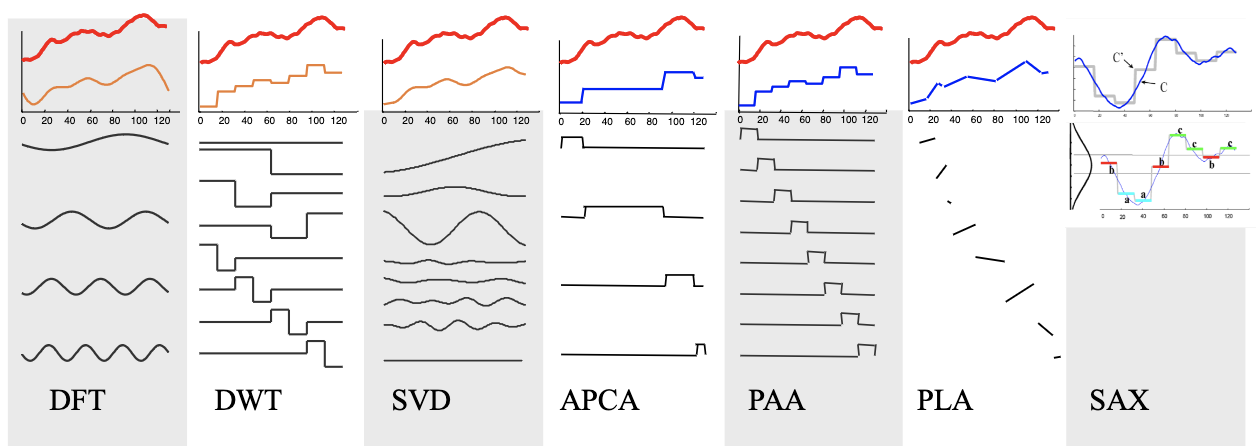
\includegraphics[width=0.8\linewidth]{img/approximations.png}
    \caption{The most common time series approximations.}
    \label{fig:approx-ts}
\end{figure}